
%% bare_jrnl.tex
%% V1.4b
%% 2015/08/26
%% by Michael Shell
%% see http://www.michaelshell.org/
%% for current contact information.
%%
%% This is a skeleton file demonstrating the use of IEEEtran.cls
%% (requires IEEEtran.cls version 1.8b or later) with an IEEE
%% journal paper.
%%
%% Support sites:
%% http://www.michaelshell.org/tex/ieeetran/
%% http://www.ctan.org/pkg/ieeetran
%% and
%% http://www.ieee.org/

%%*************************************************************************
%% Legal Notice:
%% This code is offered as-is without any warranty either expressed or
%% implied; without even the implied warranty of MERCHANTABILITY or
%% FITNESS FOR A PARTICULAR PURPOSE! 
%% User assumes all risk.
%% In no event shall the IEEE or any contributor to this code be liable for
%% any damages or losses, including, but not limited to, incidental,
%% consequential, or any other damages, resulting from the use or misuse
%% of any information contained here.
%%
%% All comments are the opinions of their respective authors and are not
%% necessarily endorsed by the IEEE.
%%
%% This work is distributed under the LaTeX Project Public License (LPPL)
%% ( http://www.latex-project.org/ ) version 1.3, and may be freely used,
%% distributed and modified. A copy of the LPPL, version 1.3, is included
%% in the base LaTeX documentation of all distributions of LaTeX released
%% 2003/12/01 or later.
%% Retain all contribution notices and credits.
%% ** Modified files should be clearly indicated as such, including  **
%% ** renaming them and changing author support contact information. **
%%*************************************************************************


% *** Authors should verify (and, if needed, correct) their LaTeX system  ***
% *** with the testflow diagnostic prior to trusting their LaTeX platform ***
% *** with production work. The IEEE's font choices and paper sizes can   ***
% *** trigger bugs that do not appear when using other class files.       ***                          ***
% The testflow support page is at:
% http://www.michaelshell.org/tex/testflow/



\documentclass[journal]{IEEEtran}
%
% If IEEEtran.cls has not been installed into the LaTeX system files,
% manually specify the path to it like:
% \documentclass[journal]{../sty/IEEEtran}






% *** CITATION PACKAGES ***
%
\usepackage{cite}
\usepackage{float}	
\usepackage{graphicx}
\usepackage{caption}
% cite.sty was written by Donald Arseneau
% V1.6 and later of IEEEtran pre-defines the format of the cite.sty package
% \cite{} output to follow that of the IEEE. Loading the cite package will
% result in citation numbers being automatically sorted and properly
% "compressed/ranged". e.g., [1], [9], [2], [7], [5], [6] without using
% cite.sty will become [1], [2], [5]--[7], [9] using cite.sty. cite.sty's
% \cite will automatically add leading space, if needed. Use cite.sty's
% noadjust option (cite.sty V3.8 and later) if you want to turn this off
% such as if a citation ever needs to be enclosed in parenthesis.
% cite.sty is already installed on most LaTeX systems. Be sure and use
% version 5.0 (2009-03-20) and later if using hyperref.sty.
% The latest version can be obtained at:
% http://www.ctan.org/pkg/cite
% The documentation is contained in the cite.sty file itself.






% *** GRAPHICS RELATED PACKAGES ***
%
\ifCLASSINFOpdf
  % \usepackage[pdftex]{graphicx}
  % declare the path(s) where your graphic files are
  % \graphicspath{{../pdf/}{../jpeg/}}
  % and their extensions so you won't have to specify these with
  % every instance of \includegraphics
  % \DeclareGraphicsExtensions{.pdf,.jpeg,.png}
\else
  % or other class option (dvipsone, dvipdf, if not using dvips). graphicx
  % will default to the driver specified in the system graphics.cfg if no
  % driver is specified.
  % \usepackage[dvips]{graphicx}
  % declare the path(s) where your graphic files are
  % \graphicspath{{../eps/}}
  % and their extensions so you won't have to specify these with
  % every instance of \includegraphics
  % \DeclareGraphicsExtensions{.eps}
\fi
% graphicx was written by David Carlisle and Sebastian Rahtz. It is
% required if you want graphics, photos, etc. graphicx.sty is already
% installed on most LaTeX systems. The latest version and documentation
% can be obtained at: 
% http://www.ctan.org/pkg/graphicx
% Another good source of documentation is "Using Imported Graphics in
% LaTeX2e" by Keith Reckdahl which can be found at:
% http://www.ctan.org/pkg/epslatex
%
% latex, and pdflatex in dvi mode, support graphics in encapsulated
% postscript (.eps) format. pdflatex in pdf mode supports graphics
% in .pdf, .jpeg, .png and .mps (metapost) formats. Users should ensure
% that all non-photo figures use a vector format (.eps, .pdf, .mps) and
% not a bitmapped formats (.jpeg, .png). The IEEE frowns on bitmapped formats
% which can result in "jaggedy"/blurry rendering of lines and letters as
% well as large increases in file sizes.
%
% You can find documentation about the pdfTeX application at:
% http://www.tug.org/applications/pdftex





% *** MATH PACKAGES ***
%
%\usepackage{amsmath}
% A popular package from the American Mathematical Society that provides
% many useful and powerful commands for dealing with mathematics.
%
% Note that the amsmath package sets \interdisplaylinepenalty to 10000
% thus preventing page breaks from occurring within multiline equations. Use:
%\interdisplaylinepenalty=2500
% after loading amsmath to restore such page breaks as IEEEtran.cls normally
% does. amsmath.sty is already installed on most LaTeX systems. The latest
% version and documentation can be obtained at:
% http://www.ctan.org/pkg/amsmath





% *** SPECIALIZED LIST PACKAGES ***
%
%\usepackage{algorithmic}
% algorithmic.sty was written by Peter Williams and Rogerio Brito.
% This package provides an algorithmic environment fo describing algorithms.
% You can use the algorithmic environment in-text or within a figure
% environment to provide for a floating algorithm. Do NOT use the algorithm
% floating environment provided by algorithm.sty (by the same authors) or
% algorithm2e.sty (by Christophe Fiorio) as the IEEE does not use dedicated
% algorithm float types and packages that provide these will not provide
% correct IEEE style captions. The latest version and documentation of
% algorithmic.sty can be obtained at:
% http://www.ctan.org/pkg/algorithms
% Also of interest may be the (relatively newer and more customizable)
% algorithmicx.sty package by Szasz Janos:
% http://www.ctan.org/pkg/algorithmicx




% *** ALIGNMENT PACKAGES ***
%
%\usepackage{array}
% Frank Mittelbach's and David Carlisle's array.sty patches and improves
% the standard LaTeX2e array and tabular environments to provide better
% appearance and additional user controls. As the default LaTeX2e table
% generation code is lacking to the point of almost being broken with
% respect to the quality of the end results, all users are strongly
% advised to use an enhanced (at the very least that provided by array.sty)
% set of table tools. array.sty is already installed on most systems. The
% latest version and documentation can be obtained at:
% http://www.ctan.org/pkg/array


% IEEEtran contains the IEEEeqnarray family of commands that can be used to
% generate multiline equations as well as matrices, tables, etc., of high
% quality.




% *** SUBFIGURE PACKAGES ***
%\ifCLASSOPTIONcompsoc
%  \usepackage[caption=false,font=normalsize,labelfont=sf,textfont=sf]{subfig}
%\else
%  \usepackage[caption=false,font=footnotesize]{subfig}
%\fi
% subfig.sty, written by Steven Douglas Cochran, is the modern replacement
% for subfigure.sty, the latter of which is no longer maintained and is
% incompatible with some LaTeX packages including fixltx2e. However,
% subfig.sty requires and automatically loads Axel Sommerfeldt's caption.sty
% which will override IEEEtran.cls' handling of captions and this will result
% in non-IEEE style figure/table captions. To prevent this problem, be sure
% and invoke subfig.sty's "caption=false" package option (available since
% subfig.sty version 1.3, 2005/06/28) as this is will preserve IEEEtran.cls
% handling of captions.
% Note that the Computer Society format requires a larger sans serif font
% than the serif footnote size font used in traditional IEEE formatting
% and thus the need to invoke different subfig.sty package options depending
% on whether compsoc mode has been enabled.
%
% The latest version and documentation of subfig.sty can be obtained at:
% http://www.ctan.org/pkg/subfig




% *** FLOAT PACKAGES ***
%
%\usepackage{fixltx2e}
% fixltx2e, the successor to the earlier fix2col.sty, was written by
% Frank Mittelbach and David Carlisle. This package corrects a few problems
% in the LaTeX2e kernel, the most notable of which is that in current
% LaTeX2e releases, the ordering of single and double column floats is not
% guaranteed to be preserved. Thus, an unpatched LaTeX2e can allow a
% single column figure to be placed prior to an earlier double column
% figure.
% Be aware that LaTeX2e kernels dated 2015 and later have fixltx2e.sty's
% corrections already built into the system in which case a warning will
% be issued if an attempt is made to load fixltx2e.sty as it is no longer
% needed.
% The latest version and documentation can be found at:
% http://www.ctan.org/pkg/fixltx2e


%\usepackage{stfloats}
% stfloats.sty was written by Sigitas Tolusis. This package gives LaTeX2e
% the ability to do double column floats at the bottom of the page as well
% as the top. (e.g., "\begin{figure*}[!b]" is not normally possible in
% LaTeX2e). It also provides a command:
%\fnbelowfloat
% to enable the placement of footnotes below bottom floats (the standard
% LaTeX2e kernel puts them above bottom floats). This is an invasive package
% which rewrites many portions of the LaTeX2e float routines. It may not work
% with other packages that modify the LaTeX2e float routines. The latest
% version and documentation can be obtained at:
% http://www.ctan.org/pkg/stfloats
% Do not use the stfloats baselinefloat ability as the IEEE does not allow
% \baselineskip to stretch. Authors submitting work to the IEEE should note
% that the IEEE rarely uses double column equations and that authors should try
% to avoid such use. Do not be tempted to use the cuted.sty or midfloat.sty
% packages (also by Sigitas Tolusis) as the IEEE does not format its papers in
% such ways.
% Do not attempt to use stfloats with fixltx2e as they are incompatible.
% Instead, use Morten Hogholm'a dblfloatfix which combines the features
% of both fixltx2e and stfloats:
%
% \usepackage{dblfloatfix}
% The latest version can be found at:
% http://www.ctan.org/pkg/dblfloatfix




%\ifCLASSOPTIONcaptionsoff
%  \usepackage[nomarkers]{endfloat}
% \let\MYoriglatexcaption\caption
% \renewcommand{\caption}[2][\relax]{\MYoriglatexcaption[#2]{#2}}
%\fi
% endfloat.sty was written by James Darrell McCauley, Jeff Goldberg and 
% Axel Sommerfeldt. This package may be useful when used in conjunction with 
% IEEEtran.cls'  captionsoff option. Some IEEE journals/societies require that
% submissions have lists of figures/tables at the end of the paper and that
% figures/tables without any captions are placed on a page by themselves at
% the end of the document. If needed, the draftcls IEEEtran class option or
% \CLASSINPUTbaselinestretch interface can be used to increase the line
% spacing as well. Be sure and use the nomarkers option of endfloat to
% prevent endfloat from "marking" where the figures would have been placed
% in the text. The two hack lines of code above are a slight modification of
% that suggested by in the endfloat docs (section 8.4.1) to ensure that
% the full captions always appear in the list of figures/tables - even if
% the user used the short optional argument of \caption[]{}.
% IEEE papers do not typically make use of \caption[]'s optional argument,
% so this should not be an issue. A similar trick can be used to disable
% captions of packages such as subfig.sty that lack options to turn off
% the subcaptions:
% For subfig.sty:
% \let\MYorigsubfloat\subfloat
% \renewcommand{\subfloat}[2][\relax]{\MYorigsubfloat[]{#2}}
% However, the above trick will not work if both optional arguments of
% the \subfloat command are used. Furthermore, there needs to be a
% description of each subfigure *somewhere* and endfloat does not add
% subfigure captions to its list of figures. Thus, the best approach is to
% avoid the use of subfigure captions (many IEEE journals avoid them anyway)
% and instead reference/explain all the subfigures within the main caption.
% The latest version of endfloat.sty and its documentation can obtained at:
% http://www.ctan.org/pkg/endfloat
%
% The IEEEtran \ifCLASSOPTIONcaptionsoff conditional can also be used
% later in the document, say, to conditionally put the References on a 
% page by themselves.




% *** PDF, URL AND HYPERLINK PACKAGES ***
%
%\usepackage{url}
% url.sty was written by Donald Arseneau. It provides better support for
% handling and breaking URLs. url.sty is already installed on most LaTeX
% systems. The latest version and documentation can be obtained at:
% http://www.ctan.org/pkg/url
% Basically, \url{my_url_here}.




% *** Do not adjust lengths that control margins, column widths, etc. ***
% *** Do not use packages that alter fonts (such as pslatex).         ***
% There should be no need to do such things with IEEEtran.cls V1.6 and later.
% (Unless specifically asked to do so by the journal or conference you plan
% to submit to, of course. )


% correct bad hyphenation here
\hyphenation{op-tical net-works semi-conduc-tor}


\begin{document}
%
% paper title
% Titles are generally capitalized except for words such as a, an, and, as,
% at, but, by, for, in, nor, of, on, or, the, to and up, which are usually
% not capitalized unless they are the first or last word of the title.
% Linebreaks \\ can be used within to get better formatting as desired.
% Do not put math or special symbols in the title.
\title{Cryptography in Hardware}
%
%
% author names and IEEE memberships
% note positions of commas and nonbreaking spaces ( ~ ) LaTeX will not break
% a structure at a ~ so this keeps an author's name from being broken across
% two lines.
% use \thanks{} to gain access to the first footnote area
% a separate \thanks must be used for each paragraph as LaTeX2e's \thanks
% was not built to handle multiple paragraphs
%

\author{Terence O'Brien,
        Ian Perry
% <-this % stops a space
\thanks{M. Shell was with the Department
of Electrical and Computer Engineering, Georgia Institute of Technology, Atlanta,
GA, 30332 USA e-mail: (see http://www.michaelshell.org/contact.html).}% <-this % stops a space
\thanks{J. Doe and J. Doe are with Anonymous University.}% <-this % stops a space
\thanks{Manuscript received April 19, 2005; revised August 26, 2015.}}

% note the % following the last \IEEEmembership and also \thanks - 
% these prevent an unwanted space from occurring between the last author name
% and the end of the author line. i.e., if you had this:
% 
% \author{....lastname \thanks{...} \thanks{...} }
%                     ^------------^------------^----Do not want these spaces!
%
% a space would be appended to the last name and could cause every name on that
% line to be shifted left slightly. This is one of those "LaTeX things". For
% instance, "\textbf{A} \textbf{B}" will typeset as "A B" not "AB". To get
% "AB" then you have to do: "\textbf{A}\textbf{B}"
% \thanks is no different in this regard, so shield the last } of each \thanks
% that ends a line with a % and do not let a space in before the next \thanks.
% Spaces after \IEEEmembership other than the last one are OK (and needed) as
% you are supposed to have spaces between the names. For what it is worth,
% this is a minor point as most people would not even notice if the said evil
% space somehow managed to creep in.



% The paper headers
\markboth{Computer Architecture CMPE 550 Special Topic Paper , December~2016}%
{Shell \MakeLowercase{\textit{et al.}}: Bare Demo of IEEEtran.cls for IEEE Journals}
% The only time the second header will appear is for the odd numbered pages
% after the title page when using the twoside option.
% 
% *** Note that you probably will NOT want to include the author's ***
% *** name in the headers of peer review papers.                   ***
% You can use \ifCLASSOPTIONpeerreview for conditional compilation here if
% you desire.




% If you want to put a publisher's ID mark on the page you can do it like
% this:
%\IEEEpubid{0000--0000/00\$00.00~\copyright~2015 IEEE}
% Remember, if you use this you must call \IEEEpubidadjcol in the second
% column for its text to clear the IEEEpubid mark.



% use for special paper notices
%\IEEEspecialpapernotice{(Invited Paper)}




% make the title area
\maketitle

% As a general rule, do not put math, special symbols or citations
% in the abstract or keywords.
\begin{abstract}
Since the beginning of recorded history, the act of procuring accurate information and utilizing it has marked the difference between those organizations which fail, and those which succeed.  Nowhere is this more evident than in adverserial situations.  The side which is able to learn the disposition of an enemy force while concealing their own is at a great advantage \cite{SunTzu}.  As history has progressed, the simple act of hiding information has ceased to be an effective option, and methods of obfuscating, or encrypting, that information has given birth to the field of cryptography.  In the modern age, cryptography is used daily by the majority of the population through the usage of ecommerce, email, or any number of secured web sites.  This ubiquitous usage has created a situation where quickly processing many crypotraphic requests at once is necessary, but by its nature, these requests are computationally expensive.  This is where hardware extensions which implement cryptography come into play.  This paper will explore the current state of cryptographic hardware, it's role in modern usage, and the required background information to understand it.
\end{abstract}

% Note that keywords are not normally used for peerreview papers.
\begin{IEEEkeywords}
IEEE, Cryptography, Information Theory.
\end{IEEEkeywords}






\section{Introduction}
% The very first letter is a 2 line initial drop letter followed
% by the rest of the first word in caps.
% 
% form to use if the first word consists of a single letter:
% \IEEEPARstart{A}{demo} file is ....
% 
% form to use if you need the single drop letter followed by
% normal text (unknown if ever used by the IEEE):
% \IEEEPARstart{A}{}demo file is ....
% 
% Some journals put the first two words in caps:
% \IEEEPARstart{T}{his demo} file is ....
% 
% Here we have the typical use of a "T" for an initial drop letter
% and "HIS" in caps to complete the first word.
\IEEEPARstart{T}{his} is the intro blahblah blahblahblahblah blahblahblahblah blahblah
blahblah blahblahblahblah blahblahblahblah blahblahblahblah blahblahblahblah blahblah


\section{History of Cryptography}



\section{Cryptography Basics}

A review of the basics of cryptography as a whole is beyond the scope of this paper.  To do that topic justice would require an entire paper in itself.  Thus, the basics of modern cryptography as it applies to an understanding of its implementation in hardware will be presented.

\subsection{Symmetric Key Encryption}

Modern cryptography hinges on the use of four main functions, symetric encryption, asymetric encryption, hashing, and random number generation.  Symetric encryption is method most often thought of when encryption is mentioned.  It is the use of a single key to both encrypt and decrypt a message.  Both user's must have the same key, and it must be shared in some fashion.  This has classically been a limiting factor in the adoption and usage of cryptography.  

In order to ensure a key as not been lost to the adversary, key sets must be periodically changed, which entails distributing entire new sets of keys, or having large tomes with predetermined keys available.  This is an enormous burden which grows roughly on the order of $n^2$, where n is the number of users.  Not only is this cost prohibitive at a certain n, but the logistics of securely transfering key material precludes it's use, particularly in the case of warfare or espionage.

Nevertheless, symetric key encryption has the advantage of being relatively less computationally expensive than its assymetric counterpart.  This results in many uses where the initial secure session is created through the use of assymetric methods, while the bulk of the data remains secure through symmetric encryption.


\subsection{Asymetric Key Encryption}

Advancements in the field brought about the creation of asymetric key encryption.  \ref{keytypes}



\begin{figure}[htbp]
	\centering
	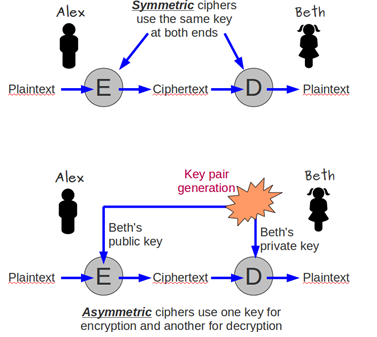
\includegraphics[width=6cm,keepaspectratio]{img/encryptionkeytypes.png}
	\caption{Encryption Key Type Breakdown \cite{KeyFigure} }
	\label{keytypes}
\end{figure}


\subsection{Hashing Functions}

Hashing functions are ubiquitous in the world of computing.  Whether they are used in common data structures such as a hash map, caching, computer graphics \cite{gpu}, or cryptography, hash functions are used in many domains for many functions.  

A hash function takes a variable length input and transforms it into a fixed length output.  This transformation is one way, and must not be able to be reversed.  Three primary uses for hashing are found in cryptography, they are used in password checking, message authentication codes \cite{hash}, and file content digesting.

When a user logs into a domain workstation, the password is not sent over the wire for authentication.  Instead, it is hashed, and that hash is compared with the stored hash.  This prevents a plaint text, or even an encrypted, password from being sent, and possibly being intercepted.  Furher, when storing passwords, the accepted method of doing so is by hashing them, as well as salting them. 

In assymetric encryption, hashing is used to check the integrity of messages, the so called authentication code.  By performing a hash of data to be encrypted, and then encrypting that hash with a private key, the recipient can decrypt the hash, verify that the data matches the hash, and then know that the user who created the hash truly sent the message.  A similar idea is used in file content digesting.  By storing the hash of a file in a public place, any user which downloads that file can perform a hash on their machine, compare it to the public hash, and ensure that the software they have downloaded is not a fake copy or has been altered in some way.

There are many hashing algorithms, but the most popular are MD5, SHA1, and SHA2, which is broken up into SHA-256 and SHA-512.  In recent times, MD5 has become less secure \cite{hashRainbow} \cite{hashBotnet}, and SHA1 is beginning to succumb to Moore's law as well.  In the very near future, SHA2 varieties will make up the bulk of cryptographic hashing.



\subsection{Random Number Generation}

One integral challenge a computer system has to achieve when doing anything with cryptography is creating truly random data.  This is extremely important, because as discussed above, cryptographic systems have been defeated simply because the random generator used to create a key wasn’t random enough.  This is a difficult challenge due to the nature of digital machines always being in well-defined, very predictable states, only changing when programs tell it to.  The best that machines like this can do is simulate randomness through algorithms that create pseudorandom numbers following mathematical procedures.  Such a set of data would look very random, but another computer following the same procedure could create the exact same sequence.  These pseudorandom numbers usually start off with a special seed value otherwise they’d always generate the same numbers.

Luckily, digital machines can look outward to the vast, chaotic universe around them for pure randomness.  One such tool that took advantage of such chaos was called Lavarand and consisted of a lava lamp with a camera.  The camera would take pictures of the lava lamp’s seemingly random blob-like movements and through computer visions algorithms output random numbers.  Such a device could then just be used to create a random seed for a pseudorandom number generator that could generate random numbers at a much higher frequency.  This example shows that randomness exists in nature and can be used for digital purposes, but is obviously limited.  

\subsection{Cryptographic Protocols}

Cryptographic protocols are security minded protocols which wrap the various cryptographic algorithms into cohesive blocks which perform all of the steps of initializing a session, encrypting, and decrypting.  Usability is of paramount importance and has been the driving factor for adoption of cryptography by common users.  Although there are many such protocols, for the purposes of this paper, onlyy SSL/TLS and HTTPS will be discussed, as they encompass the bulk of the need for hardware acceleration.

SSL/TLS, or Secure Sockets Layer/Transport Layer Security, often just called SSL, is a protocol which provides secure communications for VoIP, IM and web browsers.  When using a web browser to connect to a server over HTTPS, it is nothing more than an HTTP session over an SSL channel \cite{howSSLWorks}.  One of the key elements of this protocol is the SSL certificate.  Certificate Authorities (CA) sign certificates for domains and store their information.  When a server provides a certificate, it can be vetted against the information in the CA to ensure that the server is who it claims to be.  A great deal of trust and security is implicit in the operation of a CA, and thus has been theorized as a potential weak point by public key critics.  To date no serious breaches of a CA's operation have occured.

\begin{figure}[htbp]
	\centering
	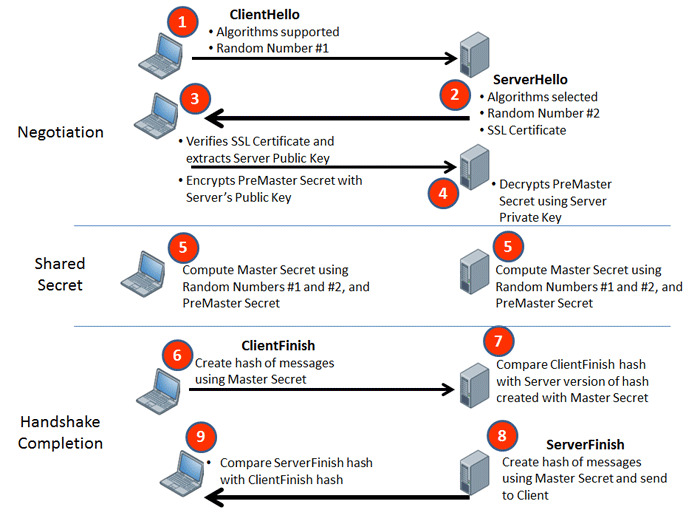
\includegraphics[width=8cm,keepaspectratio]{img/sslDiagram.png}
	\caption{SSL Process Diagram \cite{sslImage} }
	\label{sslFigure}
\end{figure}


This handshake, as the initial authentication is called, also contains information regarding the remainder of the session.  Included are details such as the TLS version, and which cipher suite will be used.  Available suites include AES, Camellia, and SEED \cite{tlsRFC}.  Available protocols for handshakes include RSA, PSK, various forms of Diffie-Helman, and others. Public-key infrastructure, which implies assymetric keys, is used for this handshake.  Further, this key protects the transmission of the Master Secret, typically an AES key, which is then in turn used to protect the actual data.  This process of assymetric keys allowing the transmission of symetric keys is the realization of overcoming the obstacle of symetric keys.  With a method of authenticating user identity, and then passing the encryption key, all of the logistical cost discussed earlier is negated.  Further, the computational cost of encrypting via AES and symetric keys is must lower than that of performing assymetric operations.  The Figure \ref{sslFigure} demonstrates the operation of SSL in a more detailed manner.

\section{Standalone Cryptographic Hardware}

In the course of using an ecommerce web page, a user may only require a single SSL session every few minutes.  This level of computation is quite low, and does not require much processing power.  Contrast this with the number of SSL connections per second that even a mid or low activity server require to service all incoming connections, and it is clear that hardware acceleration is required to alleviate the burden.  To this effect the past two decades have seen a niche market arise to provide cryptographic accelerators, as well as entire cryptographic hardware suites which take care of key management as well as algorithmic heavy lifting.

\subsection{Secure Cryptoprocessors}



\subsection{SSL Acceleration}

\subsection{Hardware Security Modules}

\section{Instruction Set Extensions}


% An example of a floating figure using the graphicx package.
% Note that \label must occur AFTER (or within) \caption.
% For figures, \caption should occur after the \includegraphics.
% Note that IEEEtran v1.7 and later has special internal code that
% is designed to preserve the operation of \label within \caption
% even when the captionsoff option is in effect. However, because
% of issues like this, it may be the safest practice to put all your
% \label just after \caption rather than within \caption{}.
%
% Reminder: the "draftcls" or "draftclsnofoot", not "draft", class
% option should be used if it is desired that the figures are to be
% displayed while in draft mode.
%
%\begin{figure}[!t]
%\centering
%\includegraphics[width=2.5in]{myfigure}
% where an .eps filename suffix will be assumed under latex, 
% and a .pdf suffix will be assumed for pdflatex; or what has been declared
% via \DeclareGraphicsExtensions.
%\caption{Simulation results for the network.}
%\label{fig_sim}
%\end{figure}

% Note that the IEEE typically puts floats only at the top, even when this
% results in a large percentage of a column being occupied by floats.


% An example of a double column floating figure using two subfigures.
% (The subfig.sty package must be loaded for this to work.)
% The subfigure \label commands are set within each subfloat command,
% and the \label for the overall figure must come after \caption.
% \hfil is used as a separator to get equal spacing.
% Watch out that the combined width of all the subfigures on a 
% line do not exceed the text width or a line break will occur.
%
%\begin{figure*}[!t]
%\centering
%\subfloat[Case I]{\includegraphics[width=2.5in]{box}%
%\label{fig_first_case}}
%\hfil
%\subfloat[Case II]{\includegraphics[width=2.5in]{box}%
%\label{fig_second_case}}
%\caption{Simulation results for the network.}
%\label{fig_sim}
%\end{figure*}
%
% Note that often IEEE papers with subfigures do not employ subfigure
% captions (using the optional argument to \subfloat[]), but instead will
% reference/describe all of them (a), (b), etc., within the main caption.
% Be aware that for subfig.sty to generate the (a), (b), etc., subfigure
% labels, the optional argument to \subfloat must be present. If a
% subcaption is not desired, just leave its contents blank,
% e.g., \subfloat[].


% An example of a floating table. Note that, for IEEE style tables, the
% \caption command should come BEFORE the table and, given that table
% captions serve much like titles, are usually capitalized except for words
% such as a, an, and, as, at, but, by, for, in, nor, of, on, or, the, to
% and up, which are usually not capitalized unless they are the first or
% last word of the caption. Table text will default to \footnotesize as
% the IEEE normally uses this smaller font for tables.
% The \label must come after \caption as always.
%
%\begin{table}[!t]
%% increase table row spacing, adjust to taste
%\renewcommand{\arraystretch}{1.3}
% if using array.sty, it might be a good idea to tweak the value of
% \extrarowheight as needed to properly center the text within the cells
%\caption{An Example of a Table}
%\label{table_example}
%\centering
%% Some packages, such as MDW tools, offer better commands for making tables
%% than the plain LaTeX2e tabular which is used here.
%\begin{tabular}{|c||c|}
%\hline
%One & Two\\
%\hline
%Three & Four\\
%\hline
%\end{tabular}
%\end{table}


% Note that the IEEE does not put floats in the very first column
% - or typically anywhere on the first page for that matter. Also,
% in-text middle ("here") positioning is typically not used, but it
% is allowed and encouraged for Computer Society conferences (but
% not Computer Society journals). Most IEEE journals/conferences use
% top floats exclusively. 
% Note that, LaTeX2e, unlike IEEE journals/conferences, places
% footnotes above bottom floats. This can be corrected via the
% \fnbelowfloat command of the stfloats package.




\section{Conclusion}
The conclusion goes here.





% if have a single appendix:
%\appendix[Proof of the Zonklar Equations]
% or
%\appendix  % for no appendix heading
% do not use \section anymore after \appendix, only \section*
% is possibly needed

% use appendices with more than one appendix
% then use \section to start each appendix
% you must declare a \section before using any
% \subsection or using \label (\appendices by itself
% starts a section numbered zero.)
%

% Can use something like this to put references on a page
% by themselves when using endfloat and the captionsoff option.
\ifCLASSOPTIONcaptionsoff
  \newpage
\fi



% trigger a \newpage just before the given reference
% number - used to balance the columns on the last page
% adjust value as needed - may need to be readjusted if
% the document is modified later
%\IEEEtriggeratref{8}
% The "triggered" command can be changed if desired:
%\IEEEtriggercmd{\enlargethispage{-5in}}

% references section

% can use a bibliography generated by BibTeX as a .bbl file
% BibTeX documentation can be easily obtained at:
% http://mirror.ctan.org/biblio/bibtex/contrib/doc/
% The IEEEtran BibTeX style support page is at:
% http://www.michaelshell.org/tex/ieeetran/bibtex/
%\bibliographystyle{IEEEtran}
% argument is your BibTeX string definitions and bibliography database(s)
%\bibliography{IEEEabrv,../bib/paper}
%
% <OR> manually copy in the resultant .bbl file
% set second argument of \begin to the number of references
% (used to reserve space for the reference number labels box)
\begin{thebibliography}{1}


\bibitem{SunTzu}
S. Tzu, "A quote from the art of war," in Good Reads, Goodreads, 2015. [Online]. Available: http://www.goodreads.com/quotes/744436-conceal-your-dispositions-and-your-condition-will-remain-secret-which. Accessed: Dec. 13, 2016.

\bibitem{KeyFigure}
ict@innovation, "File: Ict-innovation-LPI-Fig-110-3 1.png - Wikimedia commons," in Wikipedia, 2012. [Online]. Available: https://commons.wikimedia.org/wiki/File:Ict-innovation-LPI-Fig-110-31.png. Accessed: Dec. 13, 2016.

\bibitem{gpu}
G. J. van den Braak, J. Gómez-Luna, J. M. González-Linares, H. Corporaal and N. Guil, "Configurable XOR Hash Functions for Banked Scratchpad Memories in GPUs," in IEEE Transactions on Computers, vol. 65, no. 7, pp. 2045-2058, July 1 2016.
doi: 10.1109/TC.2015.2479595

\bibitem{hash}
P. Gutmann, D. Naccache and C. C. Palmer, "When hashes collide [applied cryptography]," in IEEE Security \& Privacy, vol. 3, no. 3, pp. 68-71, May-June 2005.
doi: 10.1109/MSP.2005.84

\bibitem{hashBotnet}
J. Anish Dev, "Usage of botnets for high speed MD5 hash cracking," Third International Conference on Innovative Computing Technology (INTECH 2013), London, 2013, pp. 314-320.
doi: 10.1109/INTECH.2013.6653658

\bibitem{hashRainbow}
H. Kumar et al., "Rainbow table to crack password using MD5 hashing algorithm," 2013 IEEE Conference on Information \& Communication Technologies, JeJu Island, 2013, pp. 433-439.
doi: 10.1109/CICT.2013.6558135

\bibitem{howSSLWorks}
2016 S. Corporation, "SSL by Symantec - learn how SSL works," in Symantec, 1995. [Online]. Available: https://www.symantec.com/content/en/us/enterprise/white\_papers/b-beginners-guide-to-ssl-certificates\_WP.pdf. Accessed: Dec. 14, 2016.

\bibitem{tlsRFC}
J. Salowey and A. Choudhury, “AES Galois Counter Mode (GCM) Cipher Suites for TLS,” RFC 5288, Aug. 2008.

\bibitem{sslImage}
"What is SSL?," in IdenTrustSSL. [Online]. Available: https://www.identrustssl.com/images/learn\_ssl\_diagram.gif. Accessed: Dec. 14, 2016.



\end{thebibliography}


% that's all folks
\end{document}


